\section{Background: Goal-oriented Requirements Language and Practical Reasoning}
\label{sect:background}

In this section, we first introduce our running example, after which we give a brief overview of the Goal-oriented Requirements Language (GRL)~\cite{Amyot:2010:EGM:1841349.1841356}, which is the goal modeling language we use to integrate with the argumentation framework\footnote{For simplicity's sake, we consider a slightly cut-down version of GRL. All the core elements of GRL are included but, for example, we have included only one level of contribution strength, where GRL contains different levels of positive and negative contribution. This simplification does not in any way influence the case study. Furthermore, extending the GRL part of RationalGRL to include the full set of GRL elements would be trivial.}. Next, we introduce argumentation; we discuss the \emph{practical reasoning argument scheme (PRAS)}~\cite{atkinson2007}, an argument scheme that is used to form arguments and counter-arguments about situations involving goals, and we give informal examples of how argument and counterargument can influence the status of beliefs about goals.   %This will be our starting point in the next section.

\subsection{Running example: Traffic Simulator}
\label{sect:goals:runningexample}

Our examples and case study are based on the data produced by a recent series of experiments by Schriek et al. \cite{SchriekEtal2016}, who in turn base their work on the so-called Irvine experiment~\cite{UCIworkshop}. This experiment contains a well-known design reasoning assignment in software engineering about a traffic simulator. In this assignment (see Appendix~\ref{sect:designprompt}), designers are provided with a problem description, requirements, and a description of the desired outcomes. The client of the project is Professor E, who teaches civil engineering courses at an American university. In order for the professor to teach students the various theories concerning traffic (such as queuing theory), traffic simulator software needs to be developed in which students can create visual maps of an area, regulate traffic, and so forth. Schriek et al. asked designers (groups of students) to discuss the requirements of this traffic simulator. These discussions were recorded and transcribed. We used these transcripts for an extensive case study on the basis of which we develop our RationalGRL framework. Furthermore, we also use the traffic simulator case as running examples throughout this paper. 

\subsection{Goal-oriented Requirements Language (GRL)}
\label{sect:background:grl}
GRL is a modeling language for specifying intentions, business goals, and non-functional requirements of multiple stakeholders \cite{Amyot:2010:EGM:1841349.1841356}. GRL is part of the User Requirements Notation, an ITU-T standard, that combines goals and non-functional requirements with functional and operational requirements (i.e. use case maps). GRL can be used to specify alternatives that have to be considered, decisions that have been made, and rationales for making decisions. A GRL model is a connected graph of intentional elements that optionally are part of the actors. The GRL elements and relationships used in this paper are shown in Figure~\ref{fig:grl_legend}.

\begin{figure*}[ht]
\centering
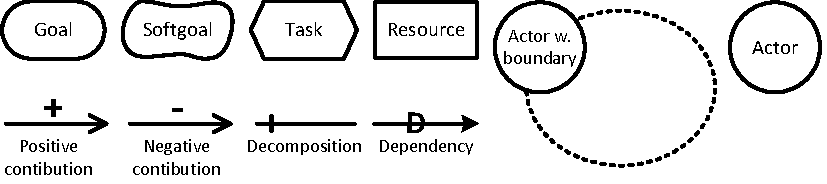
\includegraphics{img/grl_legend.pdf}
\caption{Basic elements and relationships of GRL}
\label{fig:grl_legend}
\end{figure*}


\begin{figure}[b]
\centering
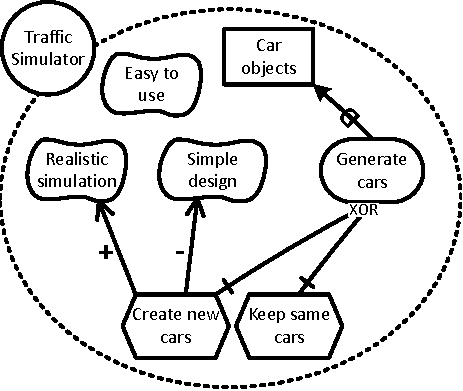
\includegraphics[width=\columnwidth]{img/Example1.pdf}
\caption{Partial GRL Model of the traffic simulator example}
\label{fig:example-small}
\end{figure} 

Figure~\ref{fig:example-small} illustrates a simplified GRL diagram from the traffic simulator design exercise. An actor represents a stakeholder of a system or the system itself (\emph{Traffic Simulator}, Figure~\ref{fig:example-small}). Actors are holders of intentions; they are the active entities in the system or its environment who want goals to be achieved, tasks to be performed, resources to be available, and softgoals to be satisfied. Softgoals differentiate themselves from goals in that there is no clear, objective measure of satisfaction for a softgoal whereas a goal is quantifiable. Softgoals (e.g. \emph{Realistic simulation}) are often related to non-functional requirements, whereas goals (such as \emph{Generate Cars}) are related to functional requirements. Tasks represent solutions to (or operationalizations of) goals and softgoals. In Figure~\ref{fig:example-small}, there are two tasks \emph{Create new cars} and \emph{Keep same cars}: in order to achieve the goal \emph{Generate cars}, the simulation can either constantly generate new ones or keep the same cars and have them reappear after they disappear off-screen. In order to be achieved or completed, softgoals, goals, and tasks may require resources to be available (e.g., \emph{Car Objects}). Finally, the full version of GRL allows design rationale to be captured using beliefs. Since we capture the reasoning and rationales behind goal models using arguments, we do not include beliefs in our simplified version of GRL (but see the discussion at the end of this section).

Different links connect the elements in a GRL model. AND, IOR (Inclusive OR), and XOR (eXclusive OR) decomposition links allow an element to be decomposed into sub-elements. In Figure~\ref{fig:example-small}, the goal \emph{Generate cars} is XOR-decomposed to the tasks \emph{Create new cars} and \emph{Keep same cars}, as they are alternative ways of achieving the goal \emph{Generate cars}. Contribution links indicate impacts of one element on another element, which can be positive or negative. Task \emph{Create new cars} has a positive contribution to the softgoal \emph{Realistic simulation}, and a negative contribution to the softgoal \emph{Simple design}. Note that the full GRL specification considers different levels of positive and negative contribution values (both quantitative and qualitative), which are not directly relevant for current purposes. Dependency links are relationships between IEs, which can model dependencies between actors. Here, the goal \emph{Generate cars} depends on the resource \emph{Car objects}. 

GRL is based on $i*$~\cite{yu1997towards} and the NFR Framework~\cite{chung2012non}, but it is less restrictive. Intentional elements and links can be more freely combined, the notion of agents is replaced with the more general notion of actors and a task does not necessarily have to be an activity performed by an actor, but may also describe properties of a solution. GRL has a well-defined syntax and semantics. Furthermore, GRL provides support for a scalable and consistent representation of multiple views/diagrams of the same goal model (see~\cite[Ch.2]{Ghanavati2013} for more details). GRL also has the capability to be extended through metadata, links, and external OCL constraints. This allows GRL to be used in many domains without the need to change the whole modeling language. For example, GRL is linked to Use Case Maps, which provides traceability between concepts and instances of the goal model and behavioral design models. Multiple views and traceability links are a good fit with our current research: we aim to add traceability links between intentional elements and their underlying arguments. 

The GRL model in Figure~\ref{fig:example-small} shows the softgoals, goals, tasks and the relationship between the different intentional elements in the model. However, the rationales and arguments behind certain intentional elements are not shown in the GRL model. Some of the questions that might be interesting to know about are the following:

\begin{itemize}
	\item Why is softgoal \emph{Easy to use} not linked to any of the goals or tasks? 
	\item What does \emph{Keep same cars} mean?
	\item Why does the task \emph{Create new cars} contribute negatively to \emph{Simple design} and positively to \emph{Realistic simulation}?
	\item Why does \emph{Generate cars} XOR-decompose into two tasks?
\end{itemize}

These are the types of the questions that we cannot answer by just looking at GRL models. The model in Figure~\ref{fig:example-small} does not contain information about discussions that led to the model, such as clarification steps for the naming, or alternatives that have been considered for the relationships. The idea behind the original GRL specification is that so-called \emph{belief} elements can be used to capture such design rationales that make later justification and review of a model easier. In the original GRL specification, however, the exact semantics of these belief elements and the ways in which they should be used remain unclear. Furthermore, belief elements cannot be attached to links between elements, which makes answering the fourth and fifth question above impossible. We further discuss belief elements in light of our proposed argumentation-based framework in Section~\ref{sect:discussions:relatedwork}. 

\subsection{Practical Reasoning Argument Scheme (PRAS)}
\label{sect:background:pras}

Reasoning about which goals to pursue and actions to take is often referred to as \emph{practical reasoning}, and has been studied extensively in philosophy and artificial intelligence. One approach is to capture practical reasoning with argument schemes~\cite{walton1990}. Applying an argument scheme results in an argument in favor of, for example, taking an action. This argument can then be tested with critical questions about, for instance, whether the action is possible given the situation, and a negative answer to such a question leads to a counterargument to the original argument for the action. 

Atkinson and Bench-Capon~\cite{atkinson2007} develop and formalize the \emph{Practical Reasoning Argument Scheme} (PRAS). A simplified version of this argument scheme is as follows:

\begin{itemize}
\item[] $G$ is a goal,
\item[] Performing action $A$ realizes goal $G$,
%\item[] Which will contribute positively to the softgoal $S$
\item[] \underline{Therefore} 
\item[] Action $A$ should be performed
\end{itemize}

Here, $G$ and $A$ are variables, which can be instantiated with concrete goals and actions to provide a specific practical argument. For example, a concrete argument about the traffic simulator is as follows: 
\begin{itemize}
\item[] \emph{Generate cars} is a goal,
\item[] Performing action \emph{Keep same cars} realizes goal \emph{Generate cars}, 
\item[] \underline{Therefore} 
\item[] Action \emph{Keep same cars} should be performed
\end{itemize}

Note that PRAS is an argument scheme that captures a full inference step: ``$G$, $A$ realizes $G$, \emph{Therefore} $A$''. There are, however, also schemes that capture simpler reasoning patterns, such as claims of the form ``$A$ does not realize $G$''. We will discuss these schemes below. 

In argumentation, conclusions which are at one point acceptable can later be rejected because of new information. For example, we may argue that, in fact, performing action \emph{Keep same cars} does not realize goal \emph{Generate cars}, thus giving a counterargument to the above instantiation of PRAS. Atkinson et al.~\cite{atkinson2007} define a set of so-called critical questions that point to typical ways in which an argument based on PRAS can be criticized. Some examples of critical questions are as follows.

\begin{enumerate}
\item[CQ1] Will the action realize the desired goal?
\item[CQ2] Are there alternative ways of realizing the same goal?
\item[CQ3] Does performing the action have a negative side effect?
\end{enumerate}

The idea is that answers to critical questions are counterarguments to the original PRAS argument. These counterarguments also follow a scheme; for example, a negative answer to CQ1 follows the scheme ``Action $A$ will not realize goal $G$'', which can be instantiated (e.g. ``\emph{Keep same cars} does not realize \emph{Generate cars''}) to form a counterargument to the original argument. 

Another way to criticize an argument for an action is to suggest an alternative action that realizes the same goal (CQ2). For example, we can argue that performing \emph{Create new cars} also realizes the goal \emph{Generate cars}. Also, it is possible that performing an action has a negative side effect (CQ3). For example, while the action \emph{Create new cars} realizes the goal \emph{Generate cars}, it has a negative side effect, namely hurting \emph{Simple design}: having the simulation constantly create new cars is fairly complex design choice. 

\begin{figure}[t]
\centering
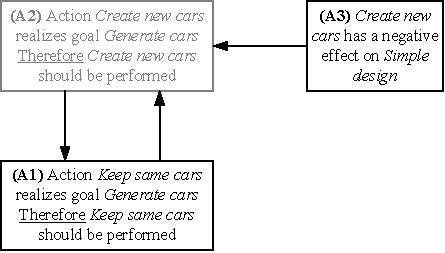
\includegraphics[]{img/fig_AF1.pdf}
\caption{PRAS arguments and attacks in the traffic simulation example.}
\label{fig:pras:example}
\end{figure}

In argumentation, counterarguments are said to \emph{attack} the original arguments. Given a set of arguments and attacks between these arguments, we can compute which arguments are accepted and which are rejected using different argumentation semantics~\cite{Dung1995}\footnote{Formal definitions of argumentation frameworks and semantics will be given in Section~\ref{sect:gmas}. In this section, we briefly discuss the intuitions behind these concepts.}. Figure \ref{fig:pras:example} shows three arguments from the traffic simulation example, where arguments are rendered as boxes and attack relations as arrows. There are two arguments based on PRAS: argument A1 for \emph{Keep Same Cars} and argument A2 for \emph{Create new cars}. Argument A2 proposes an alternative way of realizing the same goal \emph{Generate cars} with respect to argument A1 and vice versa (cf. CQ2), so A1 and A2 mutually attack each other, denoted by the arrows between A1 and A2. Argument A3 says that \emph{Create new cars} has a negative effect on \emph{Static Simulation}, so A3 attacks A2, as it points to a negative side-effect of \emph{Create new cars} (CQ3). The intuition here is that an argument is acceptable if any argument that attacks it is itself rejected. In Figure~\ref{fig:pras:example}, argument A3 is accepted because it has no attackers. This makes A2 rejected (indicated by the lighter grey color), because its attacker A3 is accepted. A1 is then also accepted, since its only attacker, A2, is rejected. 

Looking at PRAS and its critical questions, one can see how it could be used to argue about goals and actions or, more specifically, about goal models. In fact, in some of our previous work on RationalGRL \cite{vanzee-etal:renext2015,vanZee-etal:er2016} we used PRAS-arguments such as the ones above to capture reasoning about goals, and provided a translation to goal models. However, one problem of this approach is that we cannot literally use PRAS and its critical questions, as there are elements in the GRL language, such as actors and resources, which cannot be found in PRAS. Furthermore, it is not directly clear whether the critical questions as proposed by Atkinson and Bench-Capon~\cite{atkinson2007} actually apply to GRL models. In fact, our case study (Section \ref{sect:gmas}) shows that when discussing requirements, people very often do not structure their reasoning nicely in the way that PRAS presents it. That is, you do not see the discussants setting up an argument ``We have goal $G$, $A$ realizes $G$ \emph{Therefore} we should perform $A$''. A typical discussion is much more unstructured, as is clear from the transcript excerpts in Appendix~\ref{sect:transcripts:excerpts}. Thus, if we would use the version of PRAS presented in this section for our argumentation, we would violate requirement 1: The argumentation techniques must capture the actual discussions of the stakeholders or designers in the early requirements engineering phase. Our solution is to develop our own set of argument schemes and critical questions by analyzing transcripts of discussions about the traffic simulator. This set of schemes and questions and our case study are described in the next section. 

